\chapter{Graph-Datenbanken und -Frameworks - Ausgewählte Systeme }
\section{PostgreSQL}
\section{Allgemein}
\newpage
\section{Architektur}
Die Architektur von PostgresSQL ist in folgendem Bild gegeben:
\begin{center}
    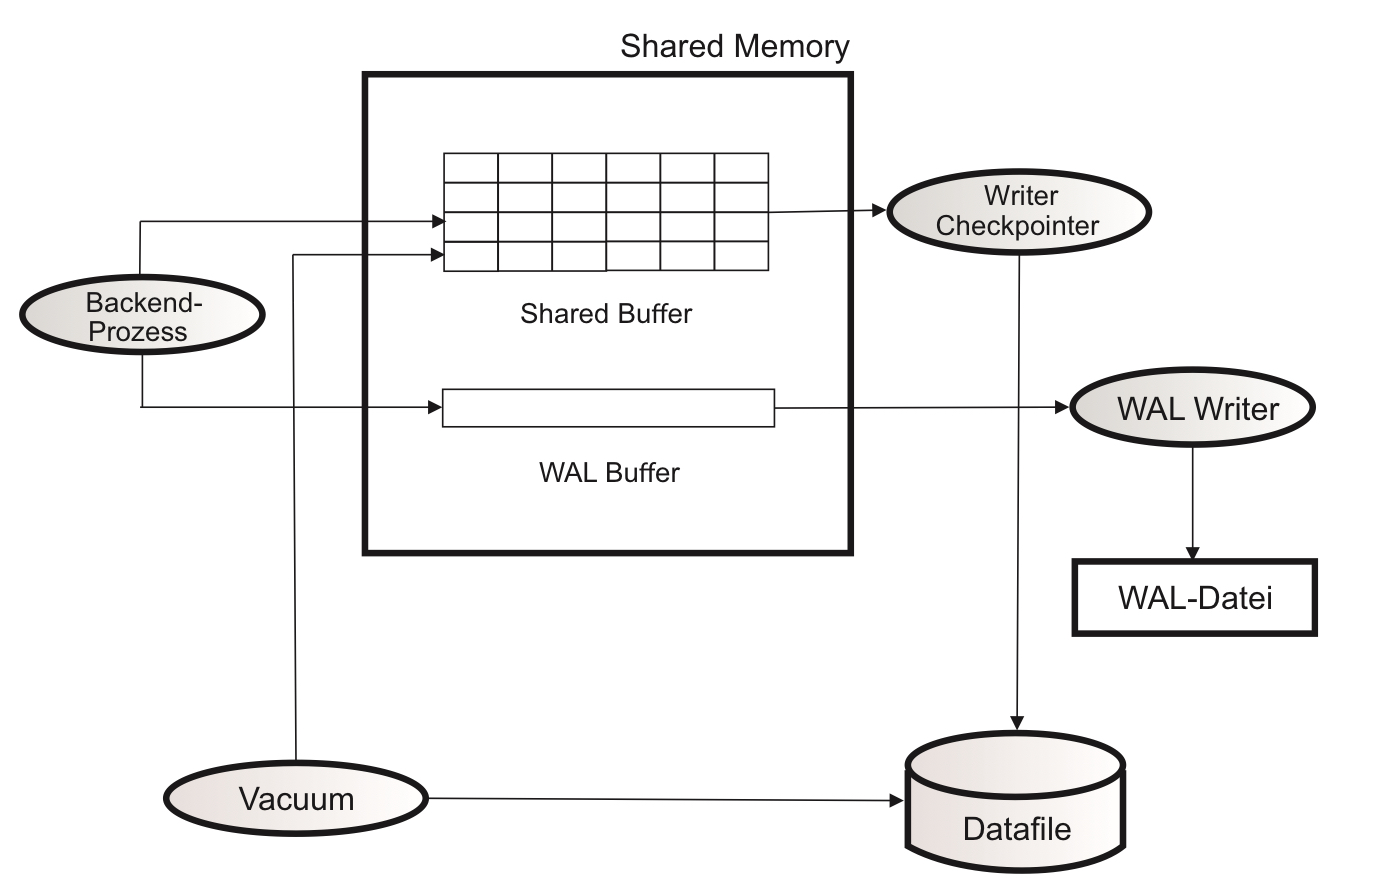
\includegraphics[width = \linewidth]{./images/PostgresSQLArchitektur.jpg}
\end{center}
Die Hauptaufgabe des Shared Buffer ist es, Input Output Operationen (I/O Operationen) auf das Datafile zu minimieren und möglichst viele Operationen im Speicher durchzuführen. Die Motivation möglichst viele Operation im Speicher durchzuführen
besteht darin, dass Operationen im Speicher schneller ausgeführt werden. Werden Operationen im Speicher ausgeführt, so werden I/O Operationen auf das Datafile reduziert. Der Writer Prozess ist für die Synchronisation
des Zustands des Shared Buffers und der Tablespaces verwantwortlich. Dieser Prozess schreibt Datenblöcke aus dem Shared Buffer auf die Tablespaces innerhalb des Datafile. Der Writer Checkpoint ist dafür verantwortlich,
dass alle geänderten Datenblöcke innerhalb des Shared Buffer in das Datafile geschrieben werden. \footnote{Vgl. \cite[Seite 26]{froehlich01}} \\
Eine PostgreSQL-Instanz wird als Server Prozess mit eigenem Datenverzeichnis und einer eigenen Konfigurationsdatei sowie einem eigenen Transaktionslog.
\section{Datenmodell}
PostgreSQL legt die Dateien im \$PGDATA-Verzeichnis ab. Wird kein Tablespace angegeben werden alle Daten im Verzeichnis Base abgelegt. Tablespaces sind in Postgres eigene Unterordner im \$PGDATA Verzeichnis.
\section{Indexe}
\section{Anfragemethoden}
\section{Konsistenz}
PostgreSQL schreibt einen Transaktionslog (Write-Ahead Log, WAL).
Dieser wird als WAL-Buffer im Arbeitsspeicher und als WAL-Dateien auf der Festplatte geführt.
Bei jedem Commit einer Transaktion wird zunächst das WAL aktualisiert bevor die Bestätigung an den Client gesendet wird.
Der walwriter-Prozess schreibt periodisch die WAL-Buffer auf die Festplatte.
